%!TEX root = ../../thesis.tex

\graphicspath{{Chapters/appendix_spider/figures/}}
\chapter{SpiderNet Found Architecture Diagrams} \label{chapter:appendix_spider}
\vspace{-1cm}
In this appendix, a few examples of SpiderNet architectures are presented to demonstrate the immense range
of structural designs afforded by the algorithm.

\section{Initial State}
For reference, all SpiderNet models start in the following state.
\begin{figure}[ht!]
    \centering
  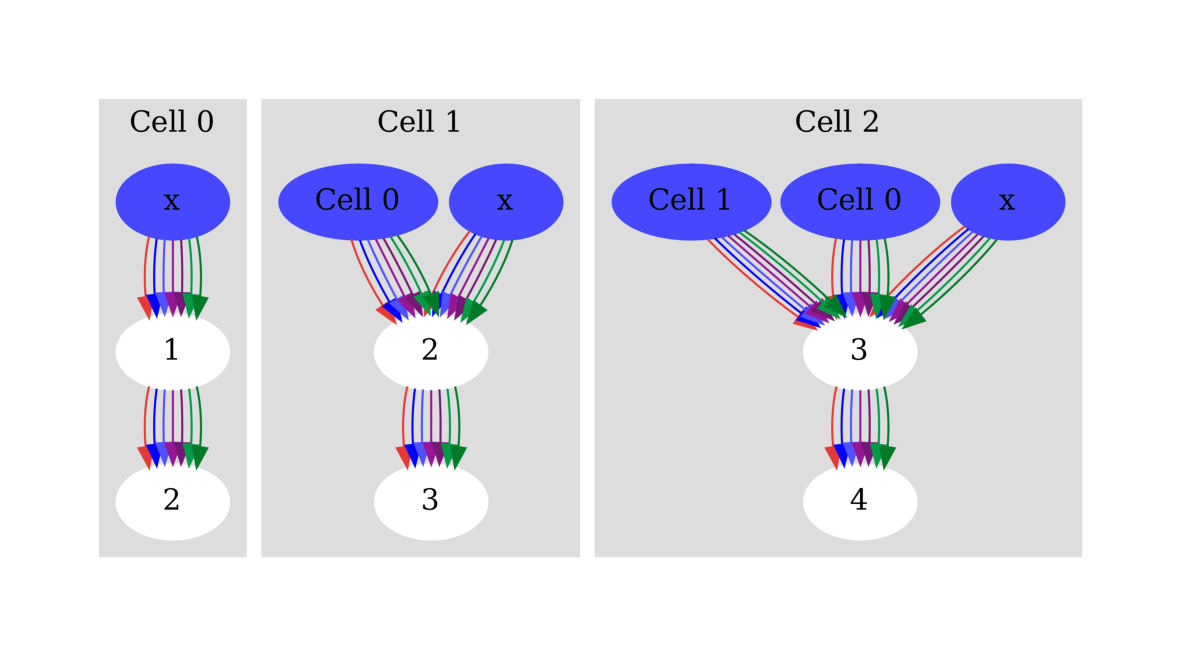
\includegraphics[width=.95\textwidth, trim={0 1cm 0 1cm}, clip]{initial_darkerblue}
    \caption[The initial state of a three cell SpiderNet model]{The initial state of a three cell SpiderNet model, with the input nodes marked in blue. The different
    colors of edges represent different operations, following the same operational color scheme used throughout
    this work.}
    \label{fig:spiderappendix_multiin_initialization}
\end{figure}

\section{SpiderNet Models}
Depicted in this section are a few SpiderNet models, generated via the Random 2 method described in
Section~\ref{sect:spider-random}. All models are displayed in the same format as the initial state diagram, with
input nodes in blue and edges color-coded by operation.

\begin{figure}[ht]
    \centering
	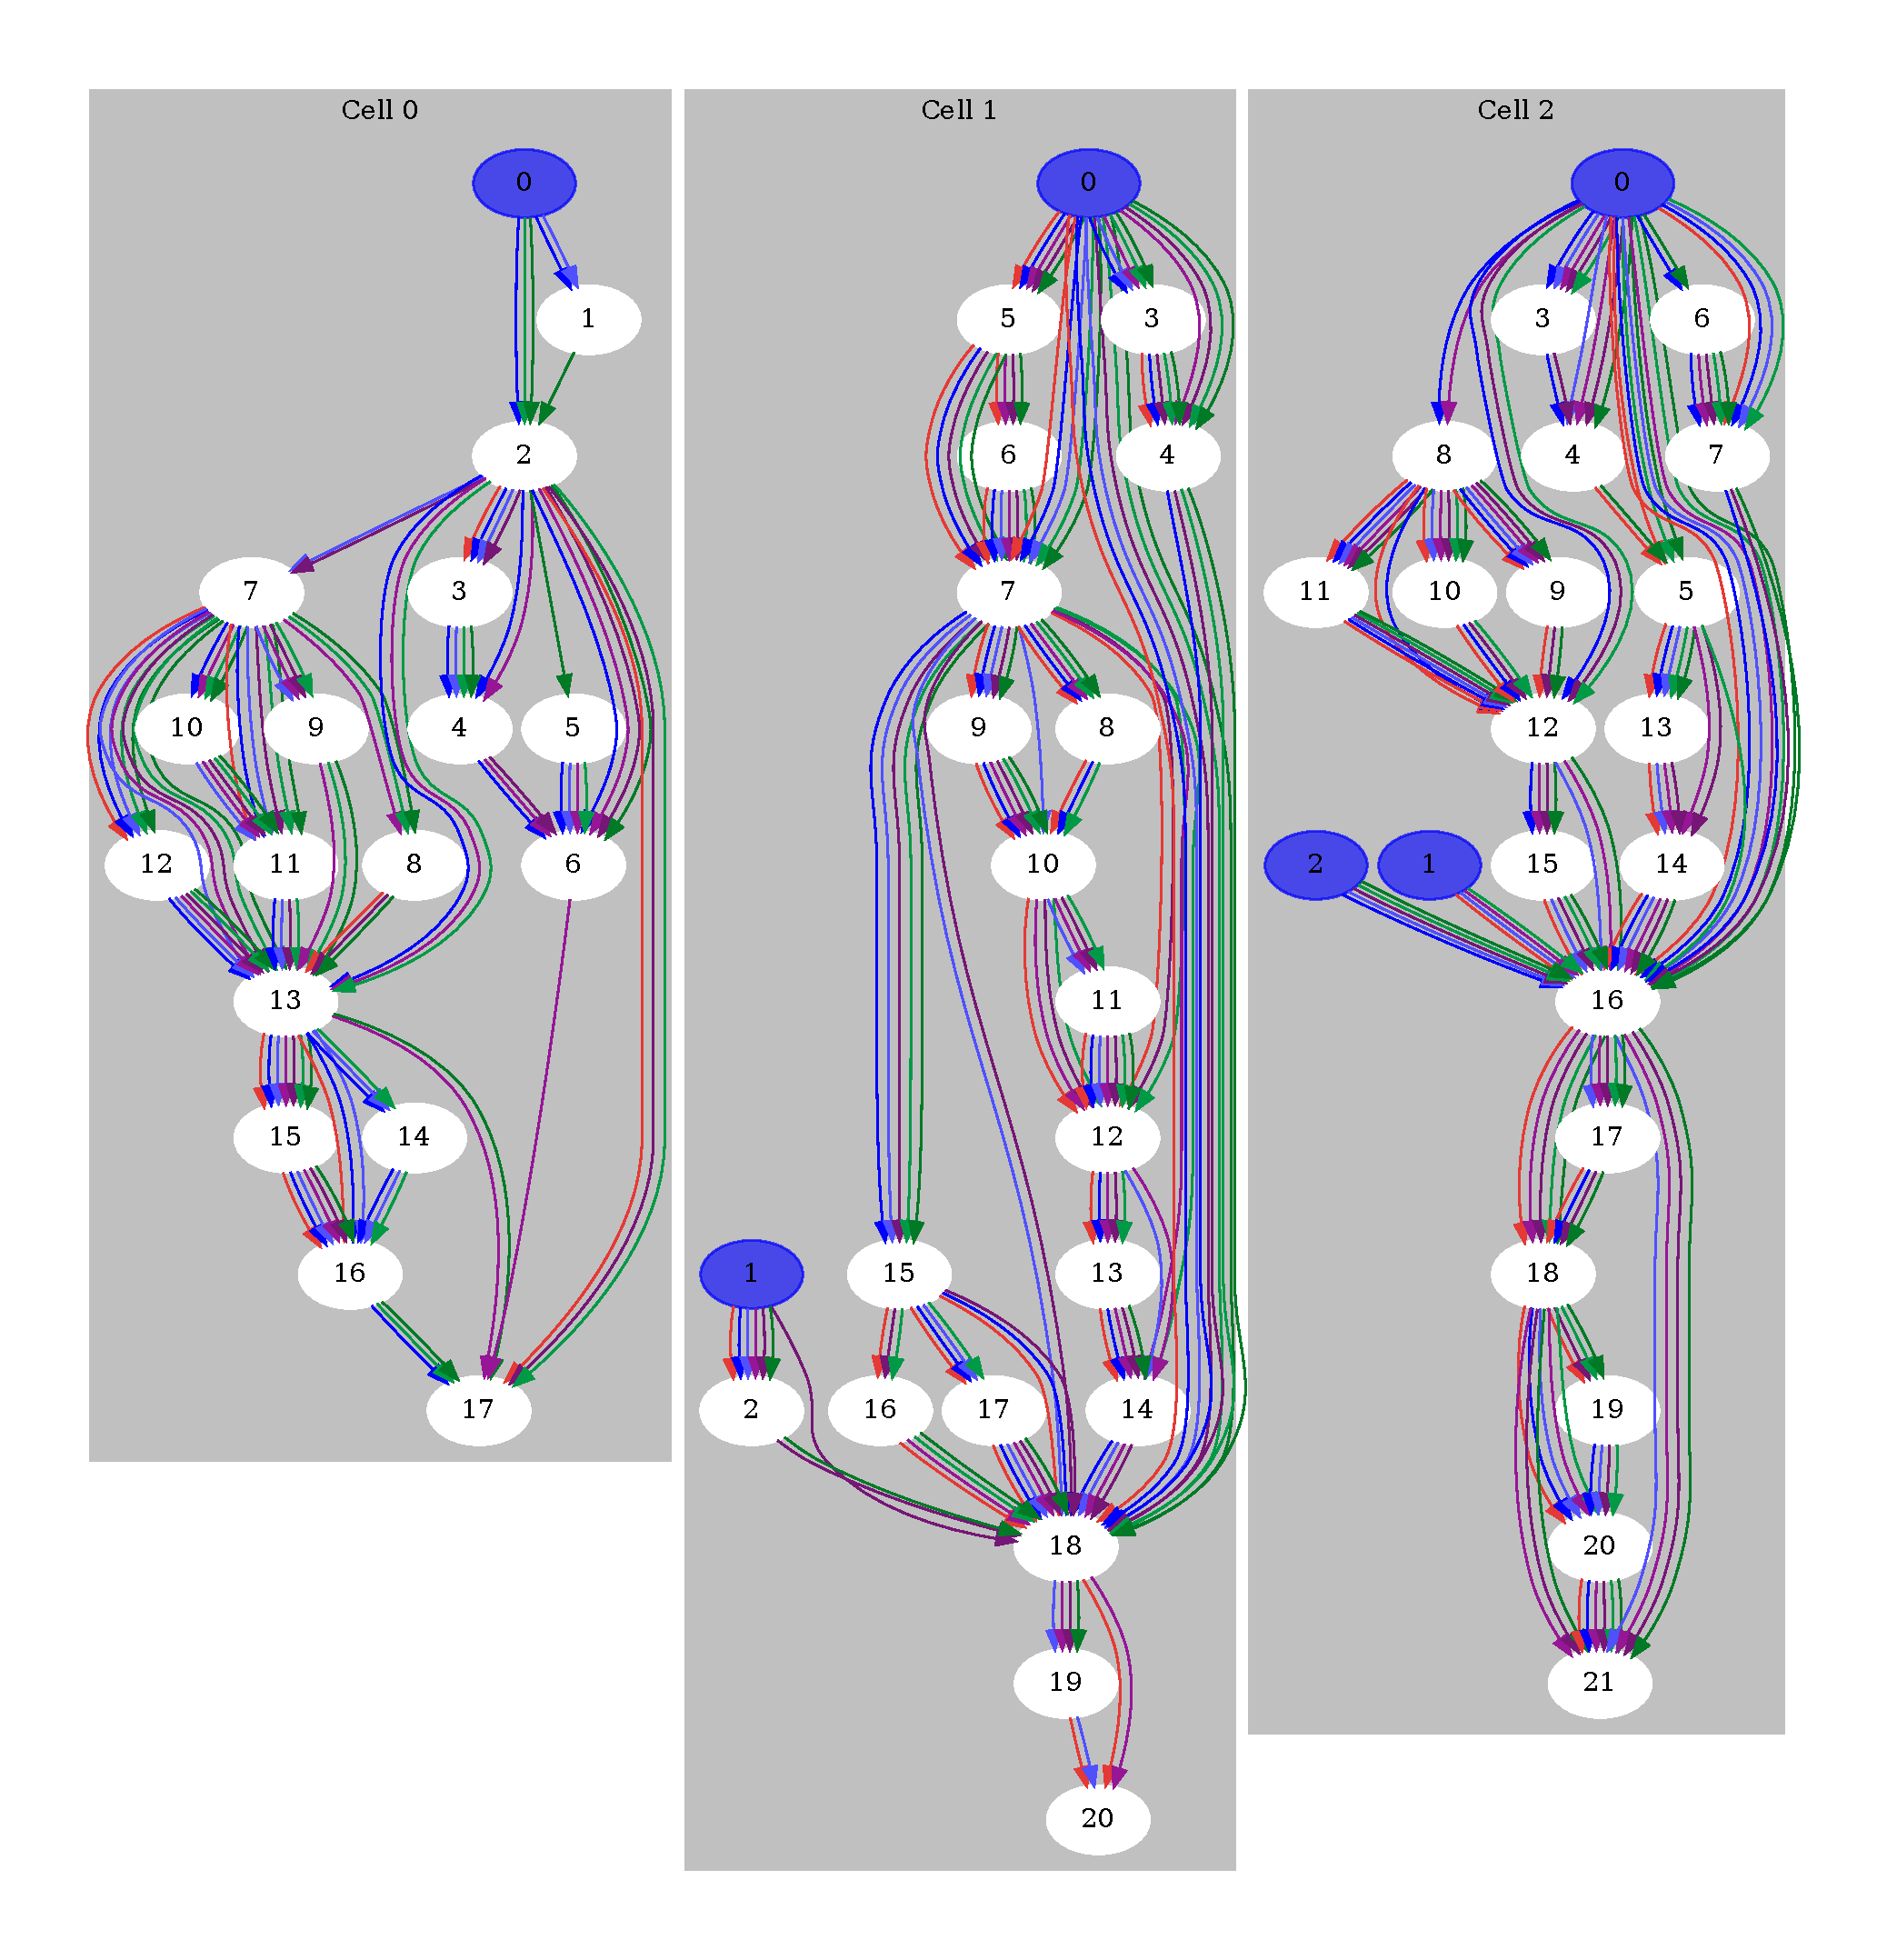
\includegraphics[width=\linewidth, trim={0 1cm 0 1cm}, clip]{random-2-1} \\
    \caption[A sample randomly grown SpiderNet model]{Model 1. Notice the bottlenecking produced by node 18 in cell 1, and node 16 in cell 2. }
    \label{fig:spider_rand0_example}
\end{figure}

\begin{figure}[ht]
    \centering
	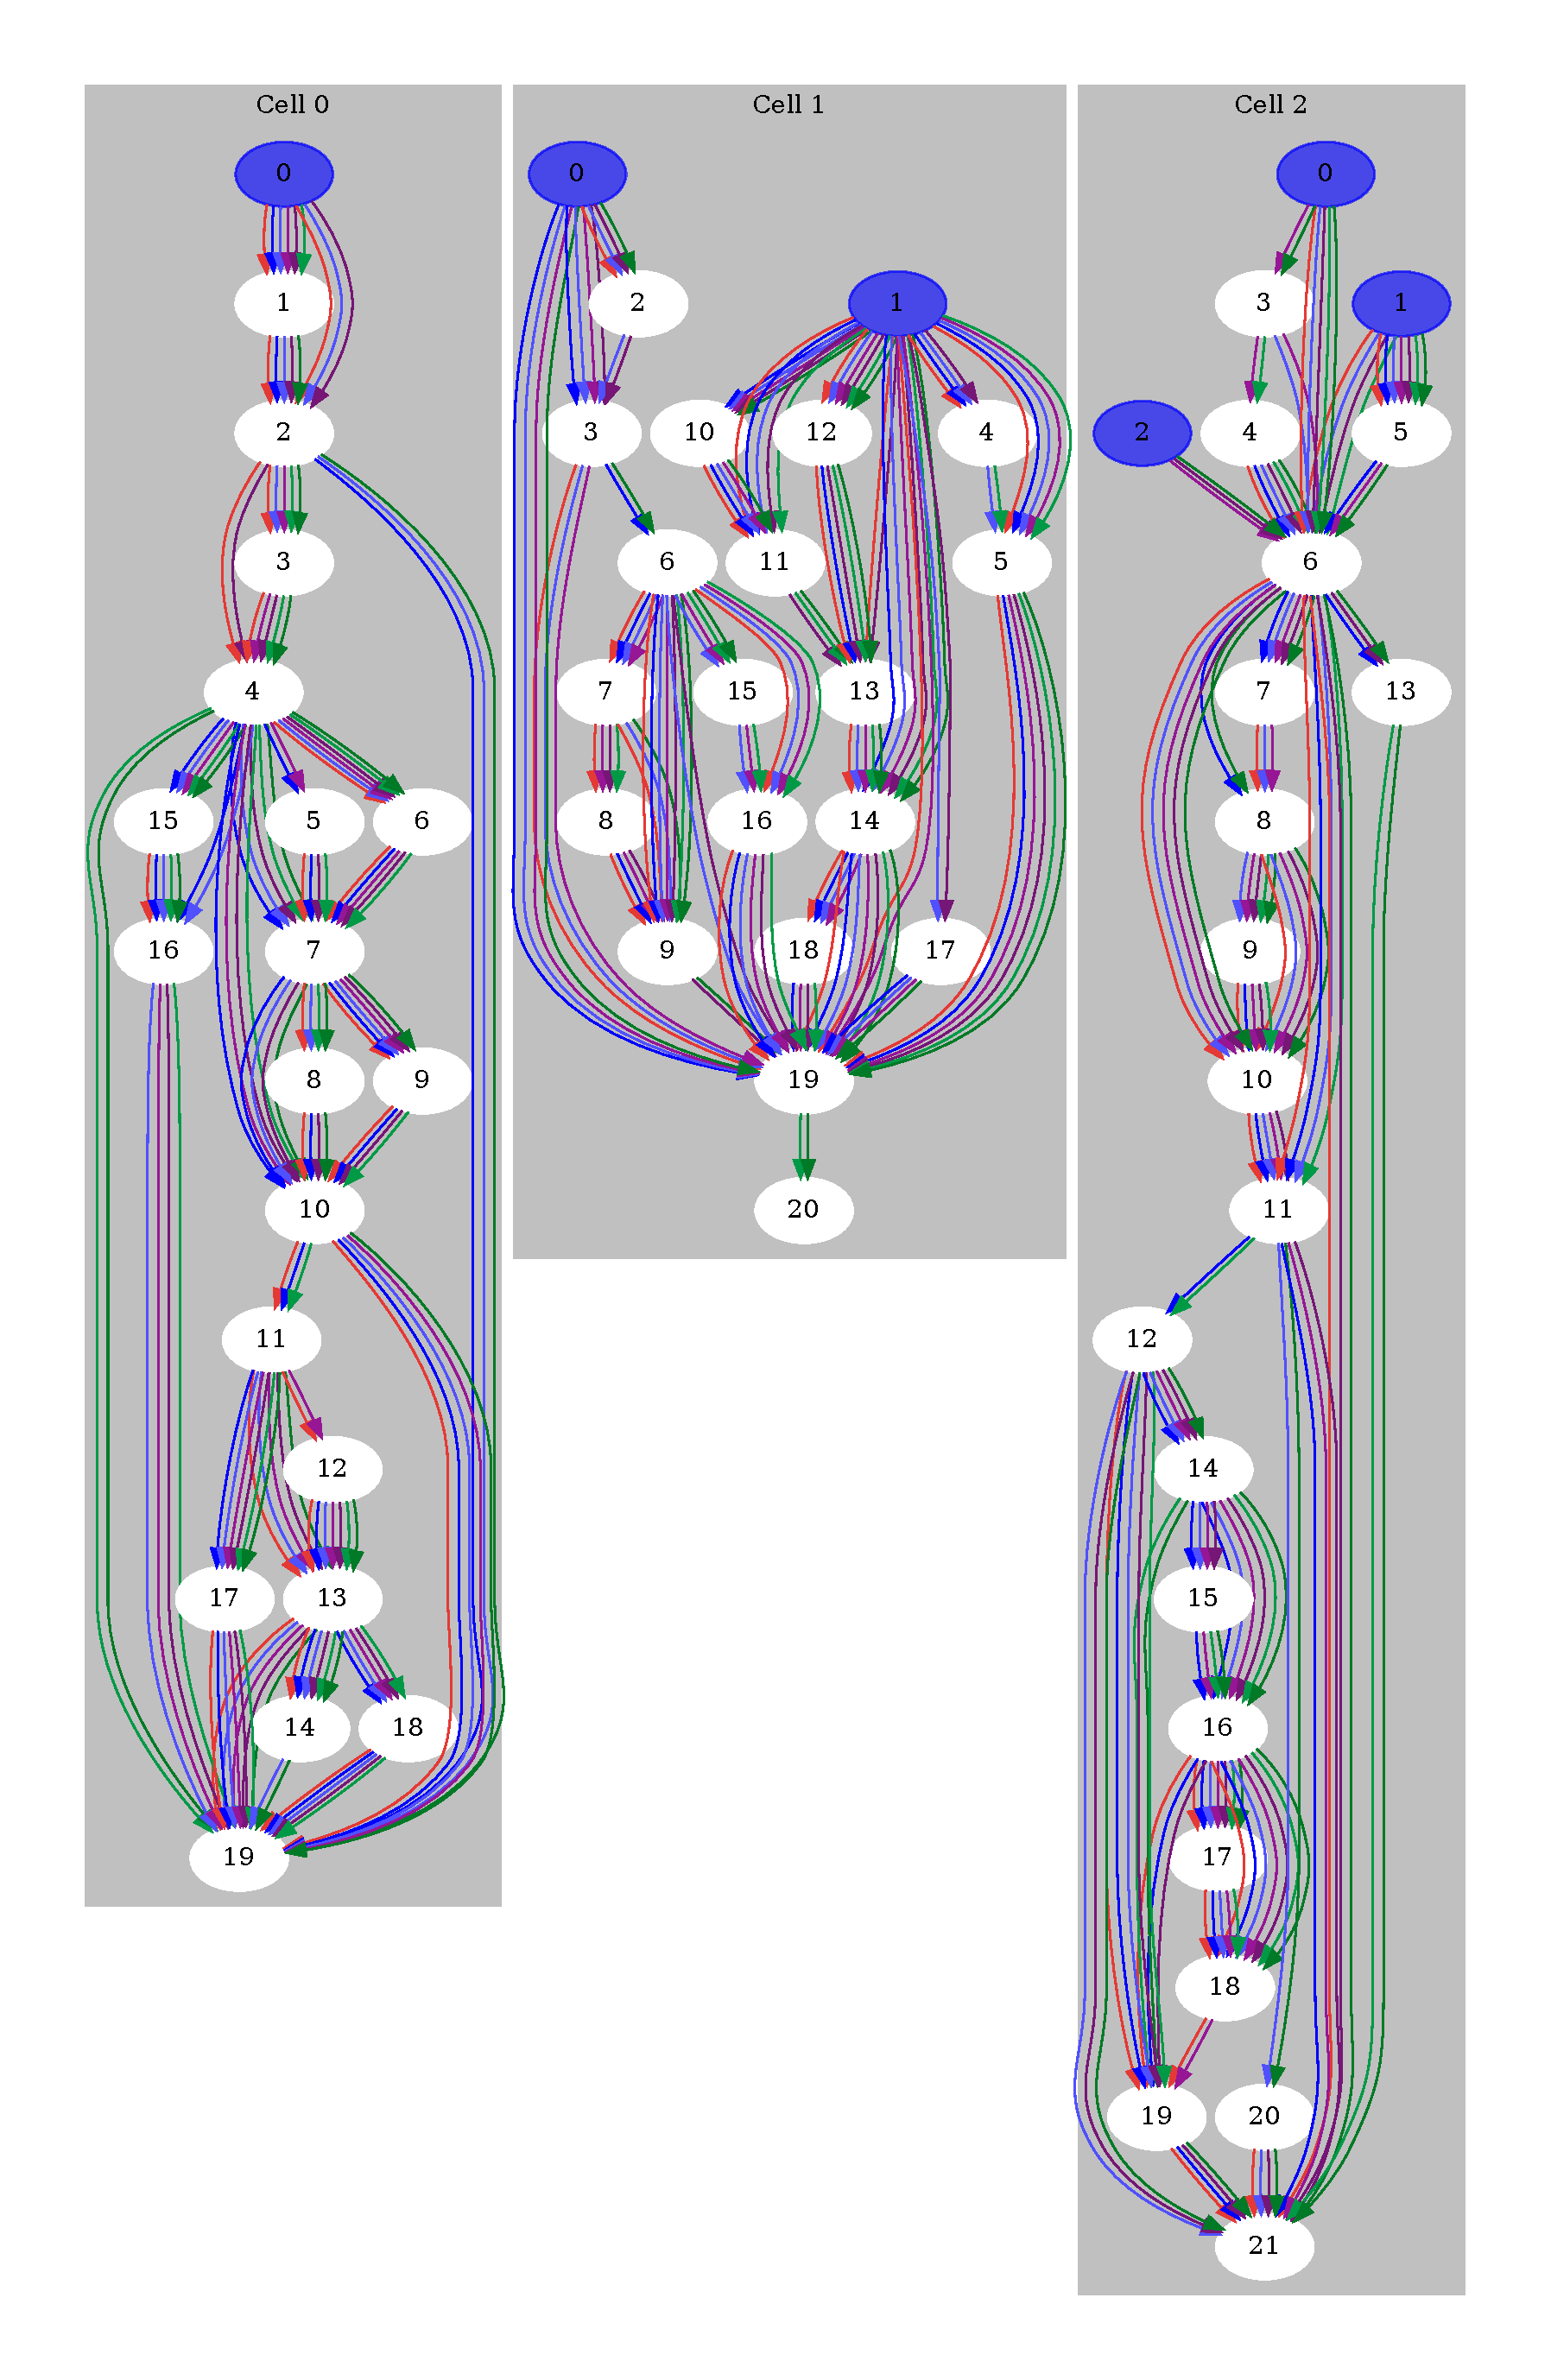
\includegraphics[width=\linewidth, trim={0 1cm 0 1cm}, clip]{random-2-2} \\
    \caption[A second randomly grown SpiderNet model]{A second randomly grown SpiderNet model.}
    \label{fig:spider_rand1_example}
\end{figure}

\begin{figure}[ht]
    \centering
	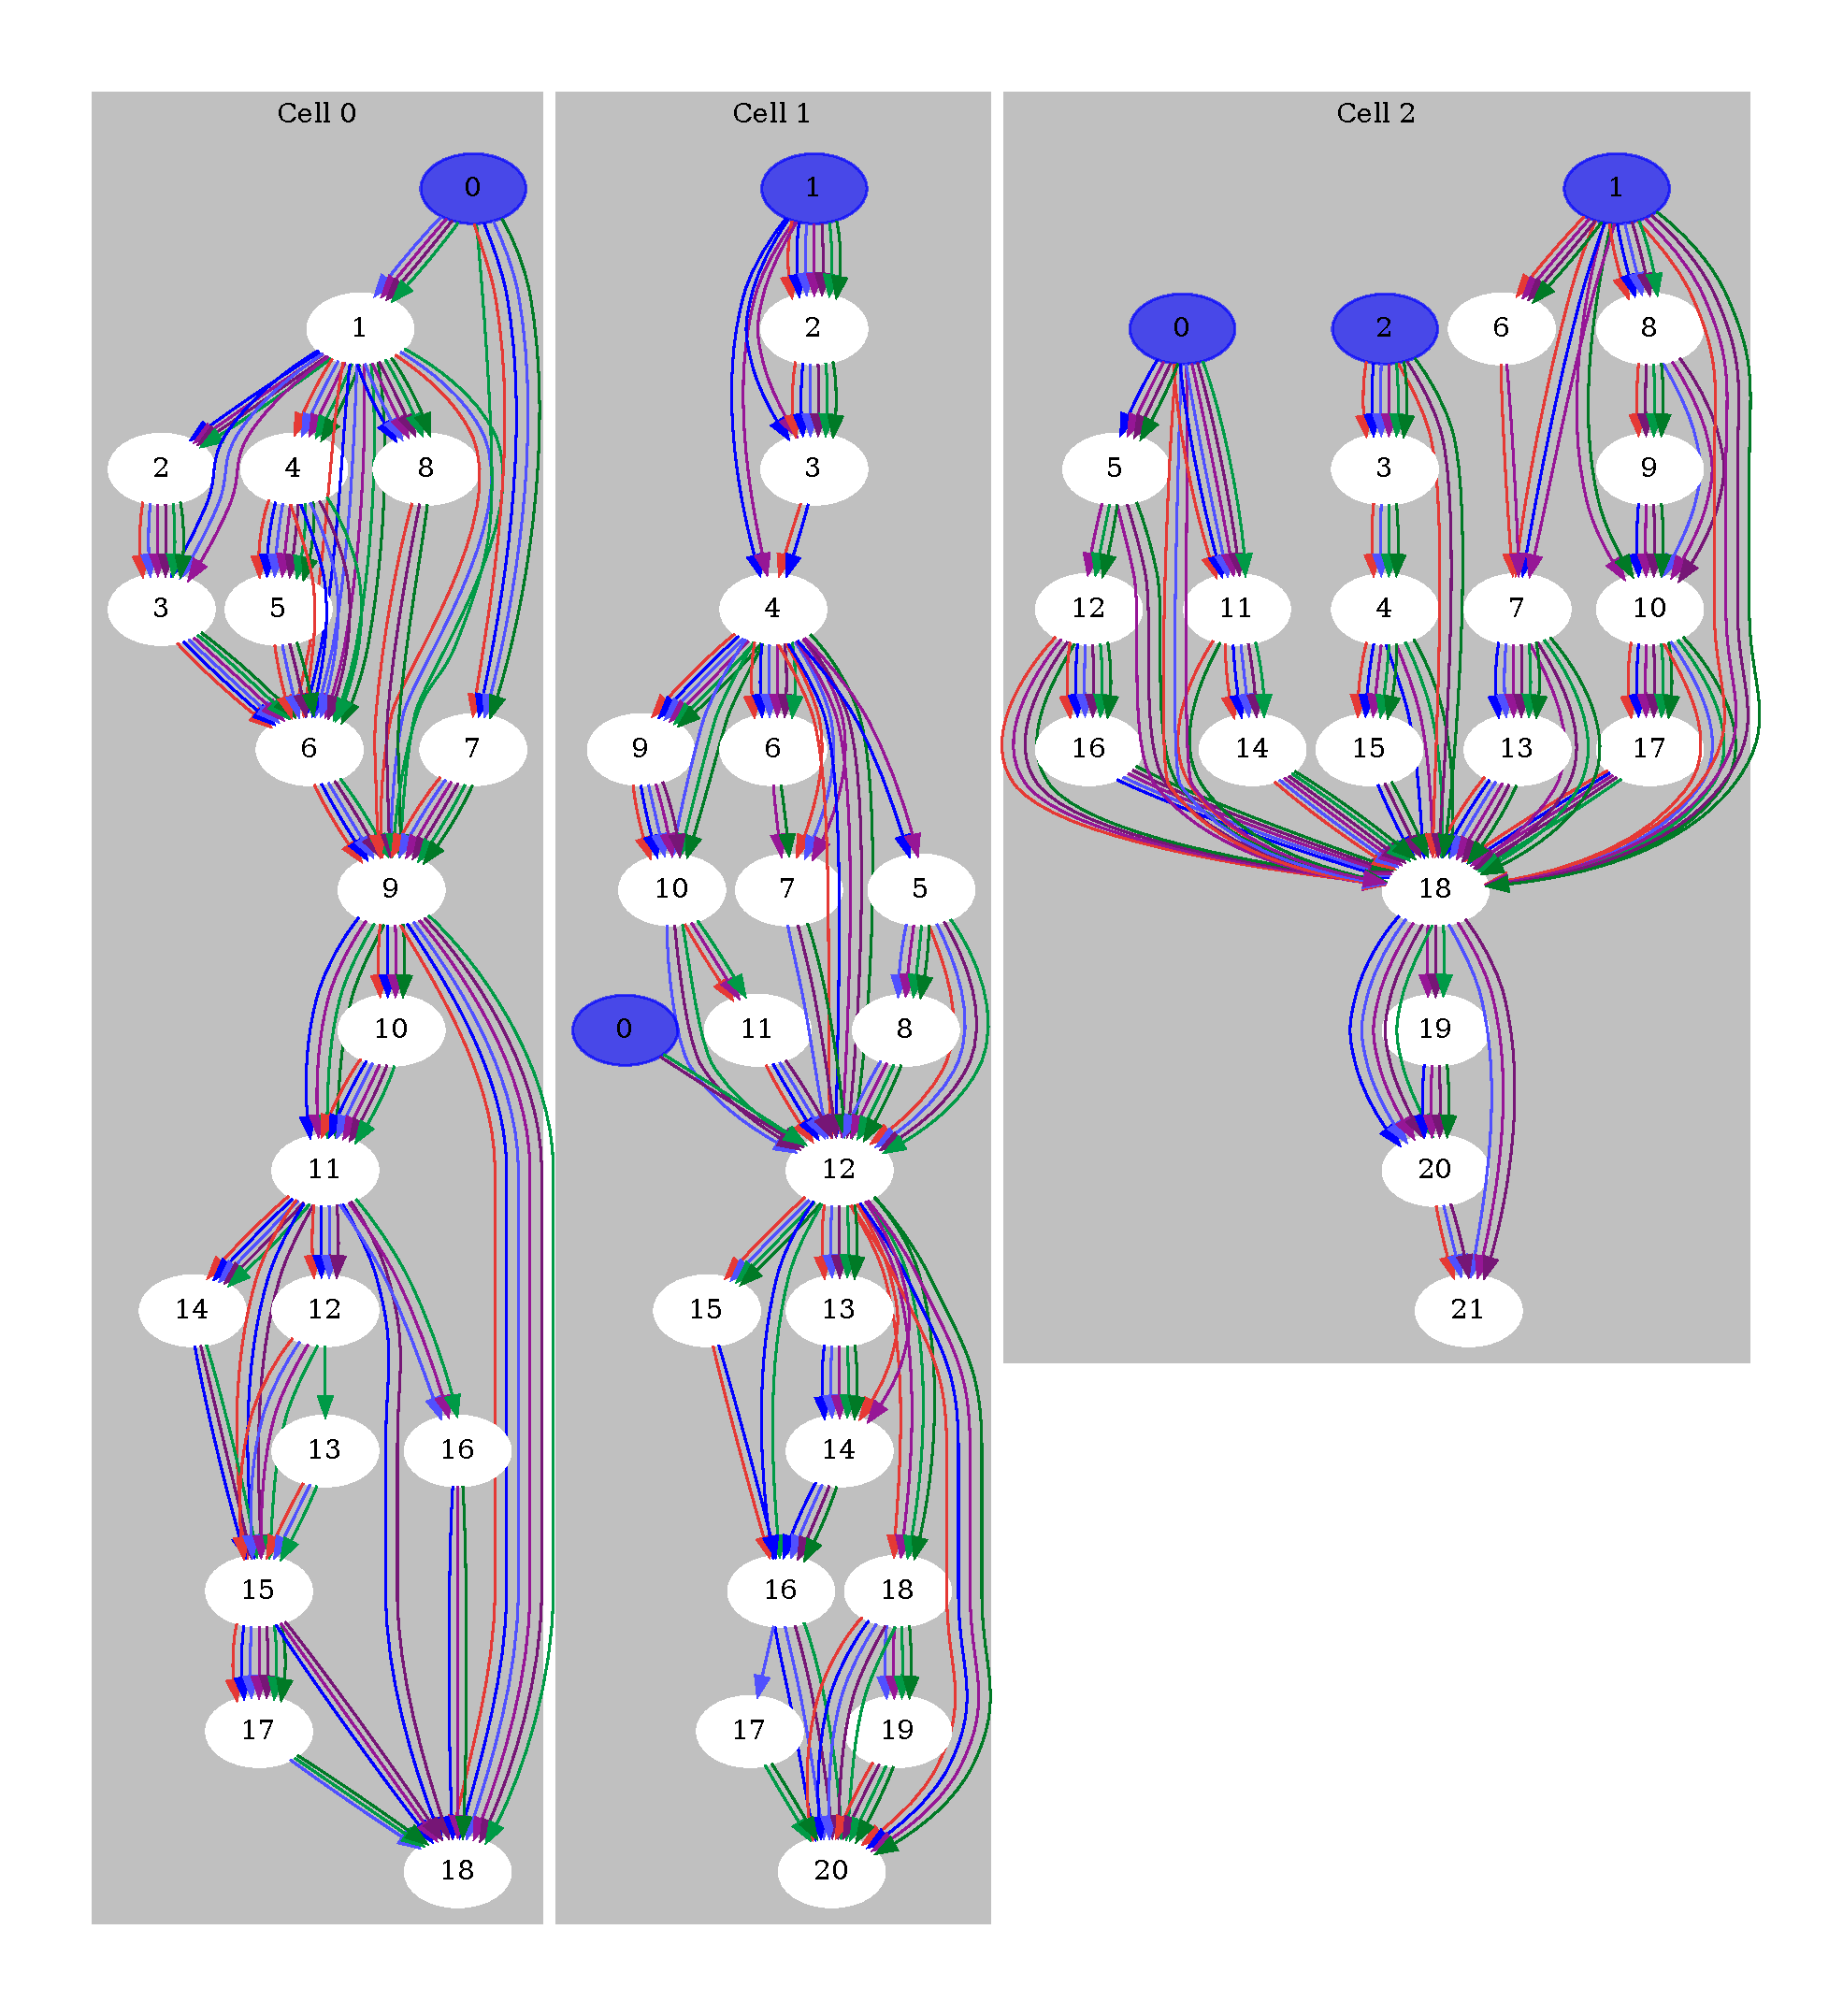
\includegraphics[width=\linewidth, trim={0 1cm 0 1cm}, clip]{random-2-3} \\
        \caption[A third randomly grown SpiderNet model]{A third randomly grown SpiderNet model.}
    \label{fig:spider_rand2_example}
\end{figure}